\chapter{Stochastic Systems, Applications}

\section{The Ornstein-Uhlenbeck Process}

We now consider one of the most important stochastic processes in science and engineering: the \textbf{Ornstein-Uhlenbeck (OU) process}. It appears in numerous contexts, from describing the velocity of a particle in a fluid (the original Langevin model) to modeling the voltage in a noisy electronic circuit. In essence, it is the canonical model for any noisy, linear system that tends to return to an equilibrium state.

The general form of the OU process is given by the SDE:
$$
dz = -\gamma z\,dt + \omega\,dW
$$
where $\gamma > 0$ is the \textit{drift} or \textit{relaxation rate}, which constantly pulls the process back towards its mean (in this case, zero), and $\omega$ is the noise intensity. This linear restoring force is what distinguishes the OU process from the free-wandering Wiener process.

\subsubsection{Solving the Ornstein-Uhlenbeck SDE}

To solve this linear SDE, we can use a technique analogous to the integrating factor method for ODEs. We define a new variable $Q(t) = e^{\gamma t}z(t)$. Our goal is to find an SDE for $Q(t)$. Using Ito's product rule (or Ito's lemma on $\psi(z,t) = e^{\gamma t}z$), we find:
\begin{align*}
    dQ &= (d(e^{\gamma t}))z + e^{\gamma t}(dz) \\
    &= (\gamma e^{\gamma t}dt)z + e^{\gamma t}(-\gamma z\,dt + \omega dW(\tau)) \\
    &= \gamma e^{\gamma t}z\,dt - \gamma e^{\gamma t}z\,dt + \omega e^{\gamma t}dW(\tau) \\
    &= \omega e^{\gamma t}dW(\tau)
\end{align*}
The drift terms have canceled perfectly, leaving a very simple SDE for $Q(t)$. We can now integrate it from 0 to $t$:
$$
Q(t) - Q(0) = \omega \int_0^t e^{\gamma \tau}dW(\tau) \quad \implies \quad Q(t) = Q(0) + \omega \int_0^t e^{\gamma \tau}dW(\tau)
$$
Substituting back $z(t) = e^{-\gamma t}Q(t)$ and $z(0) = Q(0)$, we arrive at the solution for the Ornstein-Uhlenbeck process:
$$
z(t) = z(0)e^{-\gamma t} + \omega \int_0^t e^{\gamma(\tau-t)}dW(\tau)
$$
The solution consists of two parts: a deterministic decay of the initial condition, $z(0)e^{-\gamma t}$, and a stochastic integral that represents the accumulated effect of the noise, with past noise contributions being exponentially "forgotten" over time due to the $e^{\gamma(\tau-t)}$ term.

\subsubsection{Statistical Properties}

From the solution, we can derive the key statistical properties of the OU process.

\begin{itemize}
    \item \textbf{Mean}

    Since the stochastic integral $\int e^{\gamma(\tau-t)}dW(\tau)$ has zero mean, the mean of the process is simply the deterministic part:
    $$
    \boxed{\langle z(t) \rangle = \langle z(0) \rangle e^{-\gamma t}}
    $$
    Assuming a deterministic starting point $z(0)$, the mean exponentially decays to zero, which is the equilibrium point of the system.

    \item \textbf{Variance}
    
    The variance calculation is more involved but highly instructive. Starting from our solution:
    $$
    z(t) = z(0)e^{-\gamma t} + \omega \int_0^t e^{\gamma(\tau-t)}dW(\tau)
    $$
    we can calculate the variance by expanding $\text{Var}[z(t)] = \langle z(t)^2 \rangle - \langle z(t) \rangle^2$. Since $\langle z(t) \rangle = z(0)e^{-\gamma t}$ (assuming deterministic initial condition), we have:
    $$
    \text{Var}[z(t)] = \left\langle \left( z(0)e^{-\gamma t} + \omega \int_0^t e^{\gamma(\tau-t)}dW(\tau) \right)^2 \right\rangle - z(0)^2e^{-2\gamma t}
    $$
    Expanding the square:
    \small
    $$
    \text{Var}[z(t)] = \left\langle z(0)^2e^{-2\gamma t} + 2z(0)e^{-\gamma t}\omega \int_0^t e^{\gamma(\tau-t)}dW(\tau) + \omega^2 \left(\int_0^t e^{\gamma(\tau-t)}dW(\tau)\right)^2 \right\rangle - z(0)^2e^{-2\gamma t}
    $$
    \normalsize
    The cross term vanishes since $\langle dW(\tau) \rangle = 0$, leaving:
    $$
    \text{Var}[z(t)] = \omega^2 \left\langle \left(\int_0^t e^{\gamma(\tau-t)}dW(\tau)\right)^2 \right\rangle
    $$
    
    Applying the mean, we get:
    $$
    \text{Var}[z(t)] = \omega^2 \left\langle \left(\int_0^t e^{\gamma(\tau-t)}dW(\tau)\right)^2 \right\rangle = \omega^2 \int_0^t \int_0^t e^{\gamma(\tau-t)}e^{\gamma(s-t)}\langle dW(\tau)dW(s) \rangle
    $$
    Using the property that $\langle dW(\tau)dW(s) \rangle = \delta(\tau - s)d\tau ds$, the double integral becomes:
    $$
    \text{Var}[z(t)] = \omega^2 \int_0^t \int_0^t e^{\gamma(\tau + s -2t)}\delta(s-\tau)\,ds\,d\tau  = \omega^2 \int_0^t e^{2\gamma(\tau-t)}d\tau
    $$
    Evaluating this integral:
    $$
    \text{Var}[z(t)] = \omega^2 e^{-2\gamma t} \int_0^t e^{2\gamma\tau}d\tau = \omega^2 e^{-2\gamma t} \left[ \frac{e^{2\gamma\tau}}{2\gamma} \right]_0^t = \frac{\omega^2}{2\gamma}(1 - e^{-2\gamma t})
    $$

    The total variance becomes:
    $$
    \boxed{\text{Var}[z(t)] = \text{Var}[z(0)]e^{-2\gamma t} + \frac{\omega^2}{2\gamma}(1 - e^{-2\gamma t})}
    $$
    As $t \to \infty$, the first term vanishes, and the variance approaches a constant stationary value:
    $$
    \lim_{t\to\infty} \text{Var}[z(t)] = \frac{\omega^2}{2\gamma}
    $$
    This is a crucial difference from the Wiener process, whose variance grows linearly and without bound. The restoring force in the OU process balances the diffusive effect of the noise, leading to a finite stationary variance.

    \item \textbf{Autocovariance}

    The autocovariance function for times $t$ and $q$ is defined as:
    $$
    C(t,q) = \langle (z(t) - \langle z(t) \rangle)(z(q) - \langle z(q) \rangle) \rangle
    $$
    For simplicity, let's assume the process starts at $z(0) = 0$. In this case, the mean is $\langle z(t) \rangle = 0$ for all $t$, so the autocovariance is simply the autocorrelation: $C(t,q) = \langle z(t)z(q) \rangle$.

    Using the solution for $z(t)$ with $z(0)=0$:
    $$
    z(t) = \omega \int_0^t e^{\gamma(s-t)}dW(s)
    $$
    The autocorrelation is:
    \small
    \begin{align*}
        \langle z(t)z(q) \rangle &= \left\langle \left( \omega \int_0^t e^{\gamma(s-t)}dW(s) \right) \left( \omega \int_0^q e^{\gamma(\tau-q)}dW(\tau) \right) \right\rangle \\
        &= \omega^2 e^{-\gamma(t+q)} \left\langle \int_0^t e^{\gamma s}dW(s) \int_0^q e^{\gamma \tau}dW(\tau) \right\rangle \\
        &= \omega^2 e^{-\gamma(t+q)} \int_0^t \int_0^q e^{\gamma(s+\tau)} \langle dW(s)dW(\tau) \rangle
    \end{align*}
    \normalsize
    Using the property $\langle dW(s)dW(\tau) \rangle = \delta(s-\tau)ds\,d\tau$, the double integral collapses into a single integral. We must evaluate the integral over the domain $[0,t] \times [0,q]$.
    $$
    \langle z(t)z(q) \rangle = \omega^2 e^{-\gamma(t+q)} \int_0^t \int_0^q \, e^{\gamma(\tau + s)} \delta(\tau - s) d\tau ds
    $$
    
For the evaluation of this integral, we need to consider two cases:

    \begin{itemize}
        \item \textbf{Case 1: $t \leq q$}
        
        When $t \leq q$, the domain of integration is restricted by the smaller upper limit. The delta function $\delta(\tau - s)$ forces $\tau = s$, so we integrate over the overlap region $[0, t]$:
        $$
        \langle z(t)z(q) \rangle = \omega^2 e^{-\gamma(t+q)} \int_0^t e^{2\gamma s} ds
        $$

        \vspace{-0.5em}

        Evaluating the integral:
        $$
        \langle z(t)z(q) \rangle = \omega^2 e^{-\gamma(t+q)} \left[ \frac{e^{2\gamma s}}{2\gamma} \right]_0^t = \frac{\omega^2}{2\gamma} e^{-\gamma(t+q)} (e^{2\gamma t} - 1)
        = \frac{\omega^2}{2\gamma} \left( e^{-\gamma(q-t)} - e^{-\gamma(q+t)} \right)
        $$

        \item \textbf{Case 2: $t > q$}
        
        When $t > q$, we integrate over $[0, q]$:
        $$
        \langle z(t)z(q) \rangle = \omega^2 e^{-\gamma(t+q)} \int_0^q e^{2\gamma s} ds = \frac{\omega^2}{2\gamma} \left( e^{-\gamma(t-q)} - e^{-\gamma(t+q)} \right)
        $$
    \end{itemize}

    Combining both cases, we can write the autocorrelation function as:
    $$
    \boxed{\langle z(t)z(q) \rangle = \frac{\omega^2}{2\gamma} \left( e^{-\gamma|t-q|} - e^{-\gamma(t+q)} \right)}
    $$
    For a stationary process (when $t, q \to \infty$), the second term vanishes, and we obtain the stationary autocorrelation function:
    $$
    R_z(\tau) = \lim_{t \to \infty} \langle z(t)z(t + \tau) \rangle = \frac{\omega^2}{2\gamma} e^{-\gamma|\tau|}
    $$
    where $\tau = |t-q|$ is the time lag. This autocorrelation decays exponentially with a characteristic time $1/\gamma$. In the limit of rapid relaxation ($\gamma \to \infty$), the autocorrelation function becomes sharply peaked and tends toward a Dirac delta function.
\end{itemize}

We introduce now a scaling relation between the noise intensity and the relaxation rate, by setting:
$$
\omega = c\,\gamma
$$
with $c$ a constant. Under this scaling, the SDE for $z$ becomes
$$
\dot{z} = -\gamma\,z + c\,\gamma\,\xi(t).
$$

The autocorrelation function for $z$ then reads
$$
R_z(h) = \frac{c^2}{2}\,\gamma\,e^{-\gamma|h|}, \qquad R_z(0) = \frac{c^2}{2}\,\gamma.
$$
Its total area is given by
$$
\int_{-\infty}^{+\infty} R_z(h)\,dh 
=
\int_{-\infty}^{+\infty} \frac{c^2}{2}\,\gamma\,e^{-\gamma|h|}\,dh.
=
\frac{c^2}{2}\,\gamma \cdot \frac{2}{\gamma} = c^2.
$$

For small characteristic times ($\tau=1/\gamma$ small), the autocorrelation function $R_z(h)$ approximates a white noise process:
$$
\lim_{\gamma \to \infty} R_z(h;\gamma) = c^2\,\delta(h).
$$

This derivation shows how, by choosing the scaling $\omega = c\,\gamma$, the fluctuations in the linearized dynamics around a stable equilibrium effectively become white noise in the fast relaxation limit.

\subsection{The OU Process as a Low-Pass Filter}

One of the most important interpretations of the Ornstein-Uhlenbeck process is as a \textbf{low-pass filter}. It takes a "noisy" input signal (white noise) and produces a smoother, more physically realistic output by attenuating high-frequency fluctuations. To understand this, we can analyze the process in the frequency domain using the Fourier transform.

\subsubsection{The Fourier Transform and Linear Systems}
Let $f(t)$ be a well-behaved function. Its Fourier transform, $\hat{f}(\omega)$, is defined as:
$$
\mathcal{F}[f(t)] = \hat{f}(\omega) = \int_{-\infty}^{+\infty} f(t) e^{-i\omega t} dt
$$
A key property of the Fourier transform, which can be shown using integration by parts, is how it acts on derivatives:
$$
\mathcal{F}[f'(t)] = i\omega \mathcal{F}[f(t)] = i\omega \hat{f}(\omega)
$$
This property turns differentiation in the time domain into multiplication in the frequency domain, which is extremely useful for solving linear differential equations. For example, consider a general first-order linear system with input $y(t)$ and output $f(t)$:
$$
f'(t) + \alpha f(t) = y(t)
$$
Taking the Fourier transform of the entire equation gives:
$$
i\omega\hat{f}(\omega) + \alpha\hat{f}(\omega) = \hat{y}(\omega) \quad \implies \quad \hat{f}(\omega) = \frac{\hat{y}(\omega)}{i\omega + \alpha}
$$
The term $H(\omega) = 1/(i\omega + \alpha)$ is called the \textbf{transfer function} of the system. The power of the output signal is related to the power of the input signal by the squared magnitude of the transfer function:
$$
|\hat{f}(\omega)|^2 = \frac{|\hat{y}(\omega)|^2}{\omega^2 + \alpha^2}
$$

\subsubsection{Power Spectrum of the OU Process}
We can apply this framework to the OU process, which is described by the linear SDE:
$$
\frac{dz}{dt} + \gamma z = \kappa \xi(t)
$$
Taking the Fourier transform, we get:
$$
(i\omega + \gamma)\hat{z}(\omega) = \kappa \mathcal{F}[\xi(t)] \quad \implies \quad \hat{z}(\omega) = \frac{\kappa}{i\omega + \gamma} \mathcal{F}[\xi(t)]
$$
To analyze the filtering effect, we compare the \textbf{power spectral density} of the input signal, $\xi(t)$, with that of the output signal, $z(t)$. The power spectrum is the Fourier transform of the autocorrelation function.

For the input signal (white noise), the autocorrelation is $R_{\xi}(h) = \delta(h)$ (assuming unit variance for simplicity). Its power spectrum is therefore constant:
$$
\mathcal{F}[R_{\xi}(h)] = \mathcal{F}[\delta(h)] = \int_{-\infty}^{+\infty} \delta(h) e^{-i\omega h} dh = 1
$$
This flat spectrum is why it's called "white" noise: it contains equal power at all frequencies $\omega$.

For the output signal, $z(t)$, we previously found its stationary autocorrelation function to be:
$$
R_{z}(h) = \frac{\kappa^2}{2\gamma} e^{-\gamma|h|}
$$
The power spectrum of the output is the Fourier transform of this function:
$$
\mathcal{F}[R_{z}(h)] = \frac{\kappa^2}{2\gamma} \int_{-\infty}^{+\infty} e^{-\gamma|h|} e^{-i\omega h} dh
$$
We can split the integral over positive and negative values of $h$:
$$
= \int_{-\infty}^{0} e^{(\gamma-i\omega)h}dh + \int_{0}^{+\infty} e^{-(\gamma+i\omega)h}dh = \frac{1}{\gamma-i\omega} + \frac{1}{\gamma+i\omega} = \frac{2\gamma}{\gamma^2 + \omega^2}
$$
Substituting this back, we get the output power spectrum:
$$
\mathcal{F}[R_{z}(h)] = \frac{\kappa^2}{2\gamma} \left( \frac{2\gamma}{\gamma^2 + \omega^2} \right) = \frac{\kappa^2}{\gamma^2 + \omega^2}
$$
This function, known as a \textbf{Lorentzian}, is peaked at $\omega=0$ and decays as $1/\omega^2$ for high frequencies. The OU process acts as a low-pass filter: it suppresses high-frequency components of the input white noise while allowing low-frequency components to pass through, resulting in a smoother, more physically plausible random process.

\vspace{-0.5em}
\begin{figure}[H]
    \centering
    \begin{minipage}{0.45\textwidth}
    \centering
    % Input graph: a constant function
    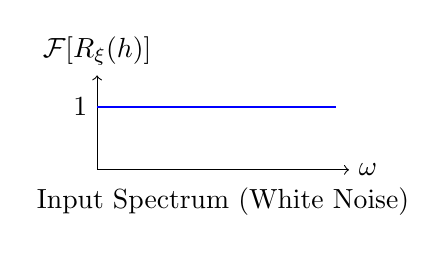
\begin{tikzpicture}[scale=0.8]
        \draw[->] (0,0) -- (4,0) node[right] {$\omega$};
        \draw[->] (0,0) -- (0,1.5) node[above] {$\mathcal{F}[R_{\xi}(h)]$};
        \draw[blue, thick] (0,1) -- (3.8,1) node[right] {};
        \node at (0,1) [left] {$1$};
        \node at (2,-0.5) {Input Spectrum (White Noise)};
    \end{tikzpicture}
    \end{minipage}
    \hfill
    \begin{minipage}{0.45\textwidth}
    \centering
    % Output graph: a Lorentzian shape
    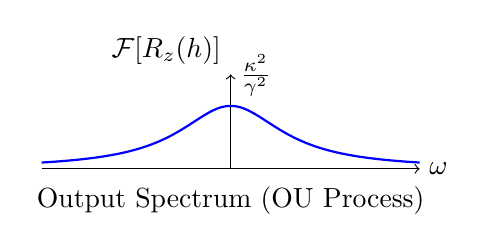
\begin{tikzpicture}[scale=0.8]
        \draw[->] (-3,0) -- (3,0) node[right] {$\omega$};
        \draw[->] (0,0) -- (0,1.5) node[above left] {$\mathcal{F}[R_{z}(h)]$};
        \draw[blue, thick, domain=-3:3, samples=100] plot (\x,{1/(1+\x*\x)});
        \node at (0,1) [above right] {$\frac{\kappa^2}{\gamma^2}$};
        \node at (0,-0.5) {Output Spectrum (OU Process)};
    \end{tikzpicture}
    \end{minipage}
    \caption{Power spectra: input white noise (flat, left) and output OU process (Lorentzian, right).}
\end{figure}

\vspace{-1em}

\subsection{Fokker-Planck equation for Ornstein-Uhlenbeck}

Given the Ito equation for the OU process:
$$
    dz = -\gamma z dt + \omega dW
$$
we can find the Fokker-Planck equation. Recalling the general form of the equation for $P(z,t)$:
$$
    \partial_t P = -\partial_z[a(z)P(z,t)] + \frac{1}{2} \partial_z^2 \left[ b(z)^2 P(z,t) \right]
$$
In our case, with $a(z) = -\gamma z$ and $b(z) = \omega$, it becomes:
$$
    \partial_t P = \partial_z(\gamma z P) + \frac{\omega^2}{2} \partial_z^2 P
$$
This equation is not simple to solve, even with the boundary conditions for a probability density:
$$
    P(\pm\infty, t) = 0 \quad \text{and} \quad \int_{\mathbb{R}} P(z, t) dz = 1
$$
These are additional conditions compared to standard PDEs and are usually of great help.

The most tractable approach is to find the stationary solution $P_s(z)$, which is the long-time limit of $P(z,t)$:
$$
    P_s(z) = \lim_{t\to\infty} P(z,t)
$$
In the stationary state, $\partial_t P = 0$, so the equation becomes an ODE:
$$
    0 = \frac{d}{dz}(\gamma z P_s) + \frac{\omega^2}{2} \frac{d^2 P_s}{d z^2}
$$
which we can rearrange to:
$$
    \frac{d^2 P_s}{d z^2} = - \frac{2\gamma}{\omega^2} \frac{d}{dz}(z P_s)
$$
Integrating once with respect to $z$, we obtain:
$$
    \frac{d P_s}{dz} = C - \frac{2\gamma}{\omega^2} z P_s(z)
$$
The boundary conditions require that $P_s(z) \to 0$ and consequently $P_s'(z) \to 0$ as $z \to \pm\infty$. For this to hold, the integration constant $C$ must be zero. This leaves us with a first-order linear ODE:
$$
    \frac{dP_s}{dz} = - \frac{2\gamma}{\omega^2} z P_s(z)
$$
The solution is a Gaussian function, which is consistent with the properties of the Ornstein-Uhlenbeck process:
$$
    P_s(z) = A e^{-\frac{\gamma}{\omega^2}z^2}
$$
This is nothing other than a Gaussian with $\mu = 0$ and $\sigma^2 = \omega^2/2\gamma$, with $A$ a constant required for normalization, namely
$$
A = \frac{1}{\sqrt{2\pi\sigma^2}}
$$

If we now consider the unperturbed system $\dot{z} = -\gamma z$, we see that the solution tends to $0$ for long times and, since it is deterministic, we obviously have
$$
P^{\mathrm{DET}}_s(z) = \delta(z)
$$
which is consistent with the perturbed case. In fact, the only equilibrium point of the deterministic case is $0$, which turns out to be the center of the Gaussian we found. Therefore, for long times, in the perturbed case, the solution will oscillate around $0$.

\section{Bistable Systems: The Ginzburg-Landau Model}

We now move from the monostable Ornstein-Uhlenbeck process to a more complex and interesting class of systems: bistable systems. These are systems that possess two stable equilibrium states. The simplest and most iconic model for such a system is the \textbf{Ginzburg-Landau equation}.

\subsubsection{The Deterministic Model}

The deterministic Ginzburg-Landau model describes the dynamics of a particle in a "double-well" potential. The equation of motion is given by:
$$
\dot{x} = x - x^3 = x(1-x)(1+x)
$$
This system has three equilibrium points, found by setting $\dot{x} = 0$:
$$
x_L = -1, \quad x_C = 0, \quad x_R = +1
$$
A simple stability analysis reveals the nature of these points:
\begin{itemize}
    \item $x_L = -1$ and $x_R = +1$ are \textbf{locally asymptotically stable}. If the system starts near one of these points, it will converge to it.
    \item $x_C = 0$ is an \textbf{unstable} equilibrium. If the system starts at this point, any infinitesimal perturbation will cause it to move away towards either $x_L$ or $x_R$.
\end{itemize}

The force $F(x) = x - x^3$ can be derived from a potential $U(x)$ where $F = -dU/dx$:
$$
U(x) = -\frac{x^2}{2} + \frac{x^4}{4}
$$
This potential has a characteristic "double-well" shape, where the stable equilibria $x_L$ and $x_R$ correspond to the minima (the "wells") of the potential, and the unstable equilibrium $x_C=0$ corresponds to the local maximum (the "barrier") between them.

If the initial condition $x(0)$ is drawn from a probability distribution $\theta(x)$, the long-term behavior of the system is deterministic. Any trajectory with $x(0) > 0$ will end up at $x_R = +1$, and any with $x(0) < 0$ will end up at $x_L = -1$. The stationary PDF will therefore consist of two Dirac delta peaks at the stable equilibria, with weights determined by the initial probability of being on either side of the unstable point:
$$
\lim_{t\to\infty} \rho(x,t) = A_R \delta(x-1) + A_L \delta(x+1)
$$
where $A_R = \text{Pr}(x_0>0)$ and $A_L = \text{Pr}(x_0<0)$.

\subsubsection{Stochastic Perturbations of the Model}

Now, let's add a stochastic white noise force to the system:
$$
\dot{x} = x - x^3 + \omega\xi(t) \quad \text{or} \quad dx = (x-x^3)dt + \omega dW_t
$$
This is a case of additive noise perturbing a conservative force. As we derived previously, the stationary probability distribution $P_s(x)$ for such a system is given by the Boltzmann distribution:
$$
P_s(x) = C \exp\left(-\frac{2}{\omega^2}U(x)\right)
$$
Substituting the Ginzburg-Landau potential $U(x) = -x^2/2 + x^4/4$, we get:
$$
P_s(x) = C \exp\left(-\frac{2}{\omega^2}\left(-\frac{x^2}{2} + \frac{x^4}{4}\right)\right) = C \exp\left(\frac{x^2}{\omega^2} - \frac{x^4}{2\omega^2}\right)
$$
where $C$ is a normalization constant. The shape of this distribution is fundamentally controlled by the noise intensity $\omega$.

% picture ?

The relationship between the potential $U(x)$ and the stationary PDF $P_s(x)$ is clear:
\begin{itemize}
    \item The stable equilibria of the deterministic system (minima of $U(x)$) become the \textbf{modes} (peaks) of the stationary PDF.
    \item The unstable equilibrium (maximum of $U(x)$) becomes the \textbf{antimode} (trough) of the stationary PDF.
\end{itemize}

The noise intensity $\omega$ determines how closely the system is confined to these potential wells:
\begin{itemize}
    \item \textbf{Weak Noise ($\omega \ll 1$):} The distribution $P_s(x)$ is sharply bimodal, with two distinct peaks centered around $x=-1$ and $x=+1$. The probability of finding the particle near the unstable point $x=0$ is extremely low. The system will exhibit small stochastic fluctuations around one of the two stable states for very long periods.
    \item \textbf{Strong Noise ($\omega \gg 1$):} The noise provides enough energy for the particle to easily cross the potential barrier between the two wells. The two peaks in the PDF broaden and merge, and the distribution becomes unimodal, centered at $x=0$. For very large $x$, the $x^4$ term still dominates, so the probability $P_s(x)$ must decay to zero.
\end{itemize}

\begin{minipage}{0.48\textwidth}
    \begin{figure}[H]
    \centering
    % PDF for small omega
    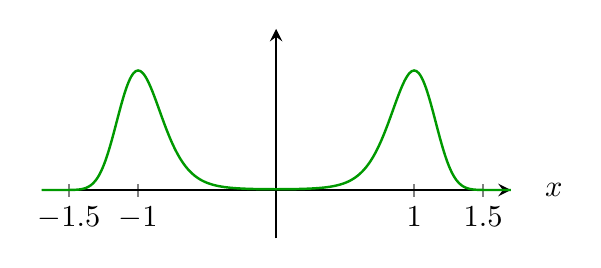
\begin{tikzpicture}[scale=1.1]
        \begin{axis}[
            width=7cm,
            height=4cm,
            domain=-1.7:1.7,
            samples=200,
            axis lines=middle,
            xlabel={$x$},
            ylabel={},
            xtick={-1.5,-1,0,1,1.5},
            ytick=\empty,
            ymin=-60, ymax=200,
            xmin=-1.7, xmax=1.7,
            every axis y label/.style={at={(ticklabel* cs:1.05)},anchor=south},
            every axis x label/.style={at={(ticklabel* cs:1.05)},anchor=west},
            axis line style=thick,
            tick style={thick}
        ]
        % Small omega: sharply bimodal
        \addplot[domain=-1.7:1.7, smooth, thick, color=green!60!black] {exp(x^2/0.1 - x^4/0.2)};
        \end{axis}
    \end{tikzpicture}
    \caption{PDF (non normalized) for small $\omega$}
    \end{figure}
\end{minipage}
\hfill
\begin{minipage}{0.48\textwidth}
    \begin{figure}[H]
    \centering
    % PDF for large omega
    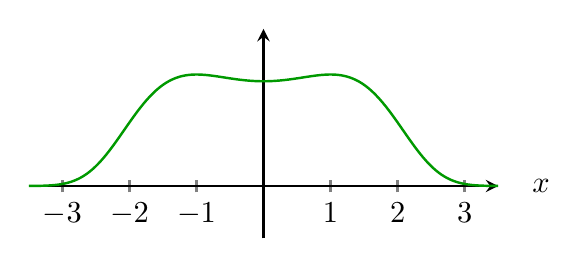
\begin{tikzpicture}[scale=1.1]
        \begin{axis}[
            width=7cm,
            height=4cm,
            domain=-3.5:3.5,
            samples=200,
            axis lines=middle,
            xlabel={$x$},
            ylabel={},
            xtick={-3,-2,-1,0,1,2,3},
            ytick=\empty,
            ymin=-0.5, ymax=1.5,
            xmin=-3.5, xmax=3.5,
            every axis y label/.style={at={(ticklabel* cs:1.05)},anchor=south},
            every axis x label/.style={at={(ticklabel* cs:1.05)},anchor=west},
            axis line style=thick,
            tick style={thick}
        ]
        % Large omega: broad, unimodal
        \addplot[domain=-3.5:3.5, smooth, thick, color=green!60!black] {exp(x^2/8 - x^4/16)};
        \end{axis}
    \end{tikzpicture}
    \caption{PDF (non normalized) for large $\omega$}
    \end{figure}
\end{minipage}

\vspace{0.5em}

This "inheritance" of stability properties from the deterministic potential to the modes of the stationary PDF is a key feature of systems with additive noise. As we will see, this direct correspondence breaks down in the presence of multiplicative noise.

\begin{observationblock}[Stochastic Miultistability]
    It is possible to say that after a very long period of time, also the first case we could see that the system moves from one peak to the other. This is due to the fact that the system is not stable and we have a non-zero probability of moving from one peak to the other. 
\end{observationblock}

\newpage

\section{Bounded Noises}

\subsection{Motivation: The Fishing Problem}

In the previous sections, we have seen how additive and multiplicative white noise can be used to model stochastic perturbations in dynamical systems. However, there are situations where the unbounded nature of Gaussian noise leads to physically unrealistic or mathematically inconsistent models. A classic example that illustrates this limitation is the problem of modeling fluctuations in fishing rates.

\subsubsection{A Population Dynamics Example}

Suppose we study a problem of fishing in the absence of fishes. Let the fish population have the following model:
$$
\dot{x} = f(x)
$$
where $x$ is the density of fishes and $f(x)$ is the net growth rate (birth rate minus death rate). Suppose now that we include fishing, which leads to a model of the type:
$$
\dot{x} = f(x) - cx
$$
with $c > 0$, of course. The fishing rate constant $c$ is really constant? No, it is very likely affected by frequent stochastic oscillations. Let us model them as a white noise perturbation:
$$
c \to c + \omega\xi(t)
$$

This gives us the stochastic differential equation:
$$
dx = f(x)dt - x(c + \omega\xi(t))dt = f(x)dt - cxdt - \omega x\xi(t)dt
$$

Converting to Ito form with $\xi(t)dt = dW(t)$:
$$
dx = [f(x) - cx]dt - \omega x dW(t)
$$

\subsubsection{The First Problem: Sign Inconsistency}

At first glance, this model seems reasonable, but it contains a fundamental flaw. The term $-\omega x dW(t)$ represents the stochastic fluctuation in the fishing rate. However, since $dW(t)$ can be positive or negative with equal probability, this term can become:
$$
-x(cdt + \omega dW) = -x(cdt + \omega\sqrt{|dt|}N(0,1))
$$

When $dW > 0$, we have increased fishing (which makes physical sense), but when $dW < 0$, we effectively have \textit{negative fishing} - which would mean we are \textbf{injecting fishes into the sea}! This is clearly unphysical.

\subsubsection{The Second Problem: Unbounded Fluctuations}

Moreover, there is a second problem: the fluctuation of the rate can become relatively large. The stochastic component $\omega\sqrt{|dt|}N(0,1)$ can easily become much larger than the deterministic fishing rate $c$. For instance, fluctuations of magnitude $10c$ or more are not rare in Gaussian processes, which would correspond to fishing rates that are an order of magnitude larger than the baseline - again, physically unrealistic.

\subsubsection{The Third Problem: Parameter Constraints}

Consider a more general nonlinear system that depends on a parameter $p$:
$$
\dot{x} = F(x,p)
$$
with the constraint that $p > 0$ for physical reasons (such as a positive fishing rate, positive resistance, positive mass, etc.). If we attempt to model fluctuations of $p$ using white noise:
$$
p \to p + \omega\xi(t)
$$

We encounter a fundamental mathematical problem: one cannot even define the model for the fluctuations of $p$ using white noise because the result of the perturbation would not be an Ito equation. The dependence of the system on $p$ is nonlinear, and Gaussian noise can make $p$ negative, violating the physical constraints of the system.

For example, consider:
$$
\dot{x} = F(x,p) \quad \text{with} \quad p = p_0 + \omega\xi(t)
$$

Since $\xi(t)$ is unbounded, there is always a non-zero probability that $p < 0$, which would make the system undefined or unphysical.

\subsubsection{The Need for Bounded Noise}

These three problems - sign inconsistency, unbounded fluctuations, and constraint violations - highlight a fundamental limitation of using unbounded Gaussian noise in certain physical systems. What we need instead are \textbf{bounded noise processes}: stochastic processes that are confined to a finite range and respect the physical constraints of the system.

The key insight is that real physical fluctuations are often naturally bounded. Fishing rates cannot be negative, electronic components have finite ranges of operation, and biological parameters typically have natural upper and lower limits. A proper stochastic model should reflect these constraints.

In the following subsections, we will explore various approaches to constructing bounded noise processes that can address these limitations while maintaining mathematical tractability.

\subsection{Recipes to generate bounded noises}

The remedy to all the above problems is "simple": one has to model the stochastic fluctuations of $p$ as follows:
$$
p \to p + \nu(t)
$$
where $\nu(t)$ is a zero-average bounded noise:
$$
\langle \nu(t) \rangle = 0
$$
$$
0 < B_l \leq p + \nu(t) \leq B_h
$$
where $B_l$ and $B_h$ depend on the model to be perturbed.

We will illustrate some simple recipes to generate bounded noises. For the sake of simplicity, we will focus only on noises such that:
$$
|\nu(t)| \leq 1
$$

\subsubsection{$1^{st}$ Recipe: Mathematical Bounded Functions}

The most straightforward approach is to apply bounded asymmetric functions to an unbounded zero mean process $y(t)$:

\begin{itemize}
    \item \textbf{Sine/Cosine functions:}
    $$
    \nu(t) = A \sin(\omega t + \phi)
    $$
    where $A \leq 1$, $\omega$ is the frequency, and $\phi$ is a random phase. This ensures $|\nu(t)| \leq A \leq 1$.
    
    \item \textbf{Tanh function:}
    $$
    \nu(t) = \tanh(\xi(t))
    $$
    where $\xi(t)$ is white noise. Since $|\tanh(x)| < 1$ for all $x$, this guarantees boundedness.
    
    \item \textbf{Arctangent function:}
    $$
    \nu(t) = \frac{2}{\pi} \arctan(\xi(t))
    $$
    This maps unbounded white noise $\xi(t)$ to the bounded interval $(-1, 1)$.
\end{itemize}

If $y(t) = W(t)$ it is better to use only periodic functions such as
$$
\nu(t) = K(W) = \sin(qW)
$$

(this noise is named 'the Sine-wiener bounded noise' in literature). Indeed, if one use a non-periodic bounded function then one gets noises whose stationary PDF tends to two Dirac deltas!

This can be easily seen by means of a specific example:

    $$
    K(W) = \begin{cases}
        z(t) & \text{if } |z(t)| \leq 1 \\
        \text{sign}(z(t)) & \text{if } |z(t)| > 1
    \end{cases}
    $$
    
Indeed $\nu(t) = K(W(t))$

$$
\text{Prob}(\nu(t) = 1) = \text{Prob}(W(t) \ge 1) = \int_1^\infty \dfrac 1{\sqrt{2\pi}t} e^{-\frac{W^2}{2t}}dW = \int_{\frac{1}{\sqrt{t}}}^{+ \infty} \dfrac 1{\sqrt{2\pi}} e^{-s^2}ds = 1 - \text{Erf}\left(\frac{1}{\sqrt{t}}\right)
$$

which tends to 1/2 for $t \to \infty$. Similarly, \text{Prob}(\nu(t) = -1) tends to 1/2.

Summarizing:
$$
\lim_{t \to \infty} P(\nu, t) = \frac{1}{2} \delta(\nu + 1) + \frac{1}{2} \delta(\nu - 1)
$$

The 'Sine-wiener bounded noise' has some interesting properties.

First, its stationary density is:
$$
P_s(\nu) = \frac{A}{\sqrt{1-\nu^2}}
$$
(and null outside $\nu \in (-1,1)$).

Second, its stationary autocovariance for large times is exponentially decreasing with characteristic time:
$$
\tau = \frac{2}{q^2}
$$

This makes it particularly useful for modeling bounded fluctuations with controllable correlation time through the parameter $q$.

\subsubsection{$2^{nd}$ Recipe: Doering-Cai-Lin Noise}

An alternative approach to generating bounded noises is through carefully designed stochastic differential equations. Consider the following family of SDEs:
$$
\begin{cases}
\dot{y}(t) = f(y) + g(y)\xi(t) & \text{(SDE with bounded support)}\\
g(\pm 1) = 0 & \text{(zero diffusion at boundaries)}\\
f(1) < 0 \qquad f(-1) > 0 & \text{(inward drift at boundaries)}\\
f(-y) = -f(y) & \text{(antisymmetric drift)}\\
g(y) > 0 \text{ for } y \in (-1,1) & \text{(positive diffusion in interior)}
\end{cases}
$$

This family defines a class of bounded noises through a clever choice of drift and diffusion coefficients. The key insight is that the boundary conditions and sign constraints ensure confinement within the interval $[-1,1]$. To see why this works, suppose that at some time $\bar{t}$ we have $y(\bar{t}) = 1$. Then the drift at the boundary becomes:
$$
\dot{y}|_{y=1} = f(1) < 0 \qquad \dot{y}|_{y=-1} = f(-1) > 0
$$

These conditions ensure that the system is always pushed away from the boundaries and back toward the interior. This guarantees that:
$$
y(t) \in [-1,1] \Rightarrow y(t) \in [-1,1].
$$

A particularly useful member of this family is obtained by choosing:
$$
f(y) = -\frac{y}{\tau} \qquad g(y) = \sqrt{\frac{\delta + 1}{\tau}}\sqrt{1 - y^2}
$$

where $\delta > -1$. This specific choice defines the Doering-Cai-Lin noise, which has the remarkable property that its stationary distribution can be calculated analytically:
$$
P_s(y) = A(1 - y^2)^{\delta}
$$

The parameter $\delta$ controls the shape of the distribution in an intuitive way: if $\delta < 0$, then the stationary PDF exhibits a 'horn-shaped' bimodal structure, while if $\delta > 0$, it becomes unimodal.

\begin{figure}[H]
    \centering
    \includegraphics[width=0.4\textwidth]{assets/doering-cai-lin.png}
    \caption{Doering-Cai-Lin noise for different values of $\delta$.}
\end{figure}

\subsubsection{$3^{rd}$ Recipe: Infinite Potential Well}

The third method for generating bounded noise draws inspiration from classical mechanics and the physics of confined motion. We consider a material point of unit mass ($m = 1$) moving in one dimension under the combined action of three distinct forces: a velocity-dependent damping force $F_d = -\gamma v$, a stochastic driving force $\omega \xi(t)$, and a confining force $F(y) = -U'(y)$ derived from a potential $U(y)$.

The crucial feature of this approach is that the confining potential becomes infinite at the boundaries, creating an impenetrable barrier. Specifically, we require:
$$
\lim_{x \to -1^+} F(x) = + \infty \qquad \lim_{x \to +1^-} F(x) = - \infty
$$

along with the potential condition:
$$
\lim_{x \to -1^+} U(x) = + \infty
$$

Under these conditions, the equation of motion becomes:
$$
\dot v = -\gamma v + F(y) + \omega \xi(t)
$$

The infinite potential walls ensure that once a particle starts within the interval, it remains forever confined there:
$$
y(0) \in (-1, 1) \Rightarrow y(t) \in (-1, 1)
$$

This mechanical perspective provides both physical intuition and mathematical rigor for understanding how bounded fluctuations can emerge from unbounded driving forces.

\begin{figure}[H]
    \centering
    \includegraphics[width=0.7\textwidth]{assets/bounded.png}
    \caption{Infinite potential well.}
\end{figure}
